% =============================================================================
% 30-bab3.tex — BAB III ANALISA DAN PERANCANGAN
% Patches: C1 (20 tabel), C3/C8 (rewrite API table), C7 (add missing tables),
%          C9 (5 auth tiers), F3 (fill requirement tables)
% =============================================================================
\chapter{ANALISA DAN PERANCANGAN}
\label{chap:analisa-perancangan}

Bab ini memaparkan proses analisis kebutuhan dan perancangan sistem yang menjadi landasan pembangunan Platform Asesmen Digital CHP. Sesuai dengan proses rekayasa perangkat lunak yang dikemukakan Sommerville (2016), aktivitas spesifikasi dan perancangan dilaksanakan secara iteratif (2016). Analisis kebutuhan mengidentifikasi apa yang harus dilakukan sistem, sedangkan perancangan mendefinisikan bagaimana sistem akan memenuhi kebutuhan tersebut.

% ─────────────────────────────────────────────────────────────────────────────
% [F3] FILLED: empty requirement tables now have content
\section{Analisis Kebutuhan Fungsional}
\label{sec:kebutuhan-fungsional}

Analisis kebutuhan fungsional mengidentifikasi fungsi-fungsi spesifik yang harus disediakan oleh sistem. Berdasarkan hasil diskusi dengan Ibu Astin selaku pemilik proyek serta observasi terhadap sistem CHP terdahulu, empat aktor utama teridentifikasi: (1) Peserta Anonim; (2) Pengguna Terdaftar; (3) Administrator; dan (4) Super Admin.

\subsection{Kebutuhan Pengguna}

Tabel~\ref{tab:kebutuhan-pengguna} menyajikan kebutuhan dari perspektif setiap aktor pengguna.

\begin{longtable}{@{}p{3cm} p{3.5cm} p{8cm}@{}}
  \caption{Kebutuhan Pengguna Platform CHP}
  \label{tab:kebutuhan-pengguna} \\
  \toprule
  \textbf{Aktor} & \textbf{Kategori} & \textbf{Kebutuhan} \\
  \midrule
  \endfirsthead
  \toprule
  \textbf{Aktor} & \textbf{Kategori} & \textbf{Kebutuhan} \\
  \midrule
  \endhead
  \bottomrule
  \endfoot
  Peserta Anonim & Asesmen & Mengambil asesmen psikologi tanpa membuat akun, melihat hasil instan, meminta laporan melalui surel \\[0.3em]
  Pengguna Terdaftar & Akun \& Riwayat & Semua fitur peserta anonim, ditambah klaim sesi anonim ke akun, riwayat asesmen, dan manajemen profil \\[0.3em]
  Administrator & Manajemen & Mengelola instrumen tes (CRUD), melihat statistik dan hasil, mengelola permintaan laporan, mengekspor data riset \\[0.3em]
  Super Admin & Keamanan & Semua fitur administrator, ditambah manajemen akun admin, aktivasi/deaktivasi pengguna, dan jejak audit \\
\end{longtable}

\subsection{Kebutuhan Perangkat Lunak}

Tabel~\ref{tab:kebutuhan-software} menyajikan kebutuhan perangkat lunak untuk pengembangan dan produksi.

\begin{table}[htbp]
  \centering
  \caption{Kebutuhan Perangkat Lunak}
  \label{tab:kebutuhan-software}
  \begin{tabularx}{\textwidth}{@{}l l X@{}}
    \toprule
    \textbf{Konteks} & \textbf{Perangkat Lunak} & \textbf{Versi/Spesifikasi} \\
    \midrule
    Pengembangan & Node.js & v22 (LTS) \\
    Pengembangan & pnpm & v9 (\textit{package manager}) \\
    Pengembangan & TypeScript & v6.0.3 (\texttt{strict: true}) \\
    Pengembangan & Git & Kontrol versi terdistribusi \\
    \textit{Framework} & Next.js & v16.2.4 (\textit{App Router}) \\
    \textit{Framework} & React & v19.2.5 (dengan \textit{React Compiler}) \\
    \textit{Framework} & tRPC & v11.16.0 \\
    ORM & Drizzle ORM & v1.0.0-beta.20 \\
    Basis Data & PostgreSQL & v17 (melalui Neon \textit{serverless}) \\
    \textit{Caching} & Upstash Redis & @upstash/ratelimit v2.0.8 \\
    Autentikasi & Auth.js (NextAuth) & v5 (next-auth 5.0.0-beta.30) \\
    Autentikasi Admin & jose & v6.2.3 (JWT mandiri) \\
    Pengujian & Vitest & v4.1.5 \\
    Pengujian & Playwright & v1.59.1 \\
    Validasi & Zod & v4.3.6 \\
    \textit{Monitoring} & Sentry & v10.50.0 \\
    Surel & Resend & v6.12.2 \\
    PDF & @react-pdf/renderer & v4.5.1 \\
    \bottomrule
  \end{tabularx}
\end{table}

\subsection{Kebutuhan Perangkat Keras}

Tabel~\ref{tab:kebutuhan-hardware} menyajikan kebutuhan perangkat keras.

\begin{table}[htbp]
  \centering
  \caption{Kebutuhan Perangkat Keras}
  \label{tab:kebutuhan-hardware}
  \begin{tabularx}{\textwidth}{@{}l l X@{}}
    \toprule
    \textbf{Konteks} & \textbf{Komponen} & \textbf{Spesifikasi} \\
    \midrule
    Server & Komputasi & Vercel \textit{serverless} (\textit{edge functions}, \textit{auto-scaling}) \\
    Server & Basis Data & Neon PostgreSQL terkelola (\textit{scale-to-zero}) \\
    Server & \textit{Cache} & Upstash Redis \textit{serverless} (API REST) \\
    Klien & Peramban & Peramban modern (Chrome, Firefox, Safari, Edge) \\
    Klien & Layar & Lebar minimum 320 px (responsif hingga 2560 px) \\
    Pengembangan & Komputer & RAM $\geq$ 8 GB, penyimpanan $\geq$ 256 GB SSD \\
    \bottomrule
  \end{tabularx}
\end{table}

\subsection{Diagram \textit{Use Case}}

Gambar~\ref{fig:use-case} menyajikan diagram \textit{use case} yang mengilustrasikan interaksi empat aktor dengan sistem.

\begin{figure}[htbp]
  \centering
  \includegraphics[width=\textwidth]{figures/gambar_3_1_use_case.png}
  \caption{Diagram \textit{Use Case} Platform Asesmen Digital CHP}
  \label{fig:use-case}
\end{figure}

Tabel~\ref{tab:kebutuhan-fungsional} merinci seluruh kebutuhan fungsional.

\begin{longtable}{@{}c p{5cm} p{3.5cm} c@{}}
  \caption{Kebutuhan Fungsional Platform CHP}
  \label{tab:kebutuhan-fungsional} \\
  \toprule
  \textbf{ID} & \textbf{Deskripsi} & \textbf{Aktor} & \textbf{Prioritas} \\
  \midrule
  \endfirsthead
  \toprule
  \textbf{ID} & \textbf{Deskripsi} & \textbf{Aktor} & \textbf{Prioritas} \\
  \midrule
  \endhead
  \bottomrule
  \endfoot
  KF-01 & Melihat katalog instrumen asesmen yang tersedia & Peserta Anonim & Tinggi \\
  KF-02 & Memulai sesi asesmen baru dengan persetujuan eksplisit & Peserta Anonim & Tinggi \\
  KF-03 & Mengisi butir soal secara bertahap dengan \textit{auto-save} & Peserta Anonim & Tinggi \\
  KF-04 & Mengirimkan jawaban dan menerima skor instan & Peserta Anonim & Tinggi \\
  KF-05 & Melihat hasil asesmen (skor total, dimensi, interpretasi) & Peserta Anonim & Tinggi \\
  KF-06 & Meminta pengiriman laporan melalui surel & Peserta Anonim & Sedang \\
  KF-07 & Registrasi akun dengan surel dan kata sandi & Pengguna Terdaftar & Tinggi \\
  KF-08 & Mengklaim sesi anonim ke akun terdaftar & Pengguna Terdaftar & Tinggi \\
  KF-09 & Melihat riwayat asesmen & Pengguna Terdaftar & Sedang \\
  KF-10 & Mengelola instrumen tes melalui CRUD & Administrator & Tinggi \\
  KF-11 & Mengonfigurasi aturan penilaian per instrumen & Administrator & Tinggi \\
  KF-12 & Melihat statistik sesi dan hasil asesmen & Administrator & Sedang \\
  KF-13 & Mengekspor data penelitian & Administrator & Sedang \\
\end{longtable}

% ─────────────────────────────────────────────────────────────────────────────
\section{Analisis Kebutuhan Non-Fungsional}
\label{sec:kebutuhan-nonfungsional}

Tabel~\ref{tab:kebutuhan-nonfungsional} menyajikan kebutuhan non-fungsional Platform CHP.

\begin{longtable}{@{}p{2cm} p{2.5cm} p{3.5cm} p{5.5cm}@{}}
  \caption{Kebutuhan Non-Fungsional Platform CHP}
  \label{tab:kebutuhan-nonfungsional} \\
  \toprule
  \textbf{Kategori} & \textbf{Parameter} & \textbf{Target Terukur} & \textbf{Strategi Implementasi} \\
  \midrule
  \endfirsthead
  \toprule
  \textbf{Kategori} & \textbf{Parameter} & \textbf{Target Terukur} & \textbf{Strategi Implementasi} \\
  \midrule
  \endhead
  \bottomrule
  \endfoot
  Performa & Waktu muat halaman & \textit{Lighthouse} $\geq$ 90 & RSC untuk mengurangi \textit{bundle} JavaScript \\[0.3em]
  Performa & Waktu respons API & $\leq$ 500 ms (P95) & \textit{Serverless edge functions} Vercel \\[0.3em]
  Keamanan & OWASP & Mitigasi A01, A02, A03, A07 & \textit{Parameterized queries}, JWT, RBAC, \textit{rate limiting} \\[0.3em]
  Keamanan & Privasi data & Kepatuhan UU PDP & Sesi anonim, IP di-\textit{hash}, surel dienkripsi AES-256-GCM \\[0.3em]
  Skalabilitas & Beban konkuren & $\geq$ 100 sesi simultan & Arsitektur \textit{serverless} \\[0.3em]
  Kegunaan & Aksesibilitas & \textit{Lighthouse} $\geq$ 95 & Semantik HTML5, kontras WCAG 2.1 AA \\[0.3em]
  Kegunaan & Responsivitas & 320 px--2560 px & Desain \textit{mobile-first} \\[0.3em]
  Keandalan & Ketersediaan & \textit{Uptime} $\geq$ 99.9\% & Infrastruktur terkelola Vercel + Neon \\[0.3em]
  Keandalan & Integritas data & Nol kehilangan data & Properti ACID, operasi atomik \\[0.3em]
  Pemeliharaan & Kualitas kode & Nol \textit{error} ESLint + TypeScript \textit{strict} & \textit{Pipeline} CI/CD dengan \textit{quality gates} \\
\end{longtable}

% ─────────────────────────────────────────────────────────────────────────────
\section{Perancangan Arsitektur Sistem}
\label{sec:arsitektur-sistem}

Gambar~\ref{fig:komponen} menyajikan diagram komponen yang memperluas Gambar~\ref{fig:arsitektur-3-tier} dengan menunjukkan modul-modul spesifik.

\begin{figure}[htbp]
  \centering
  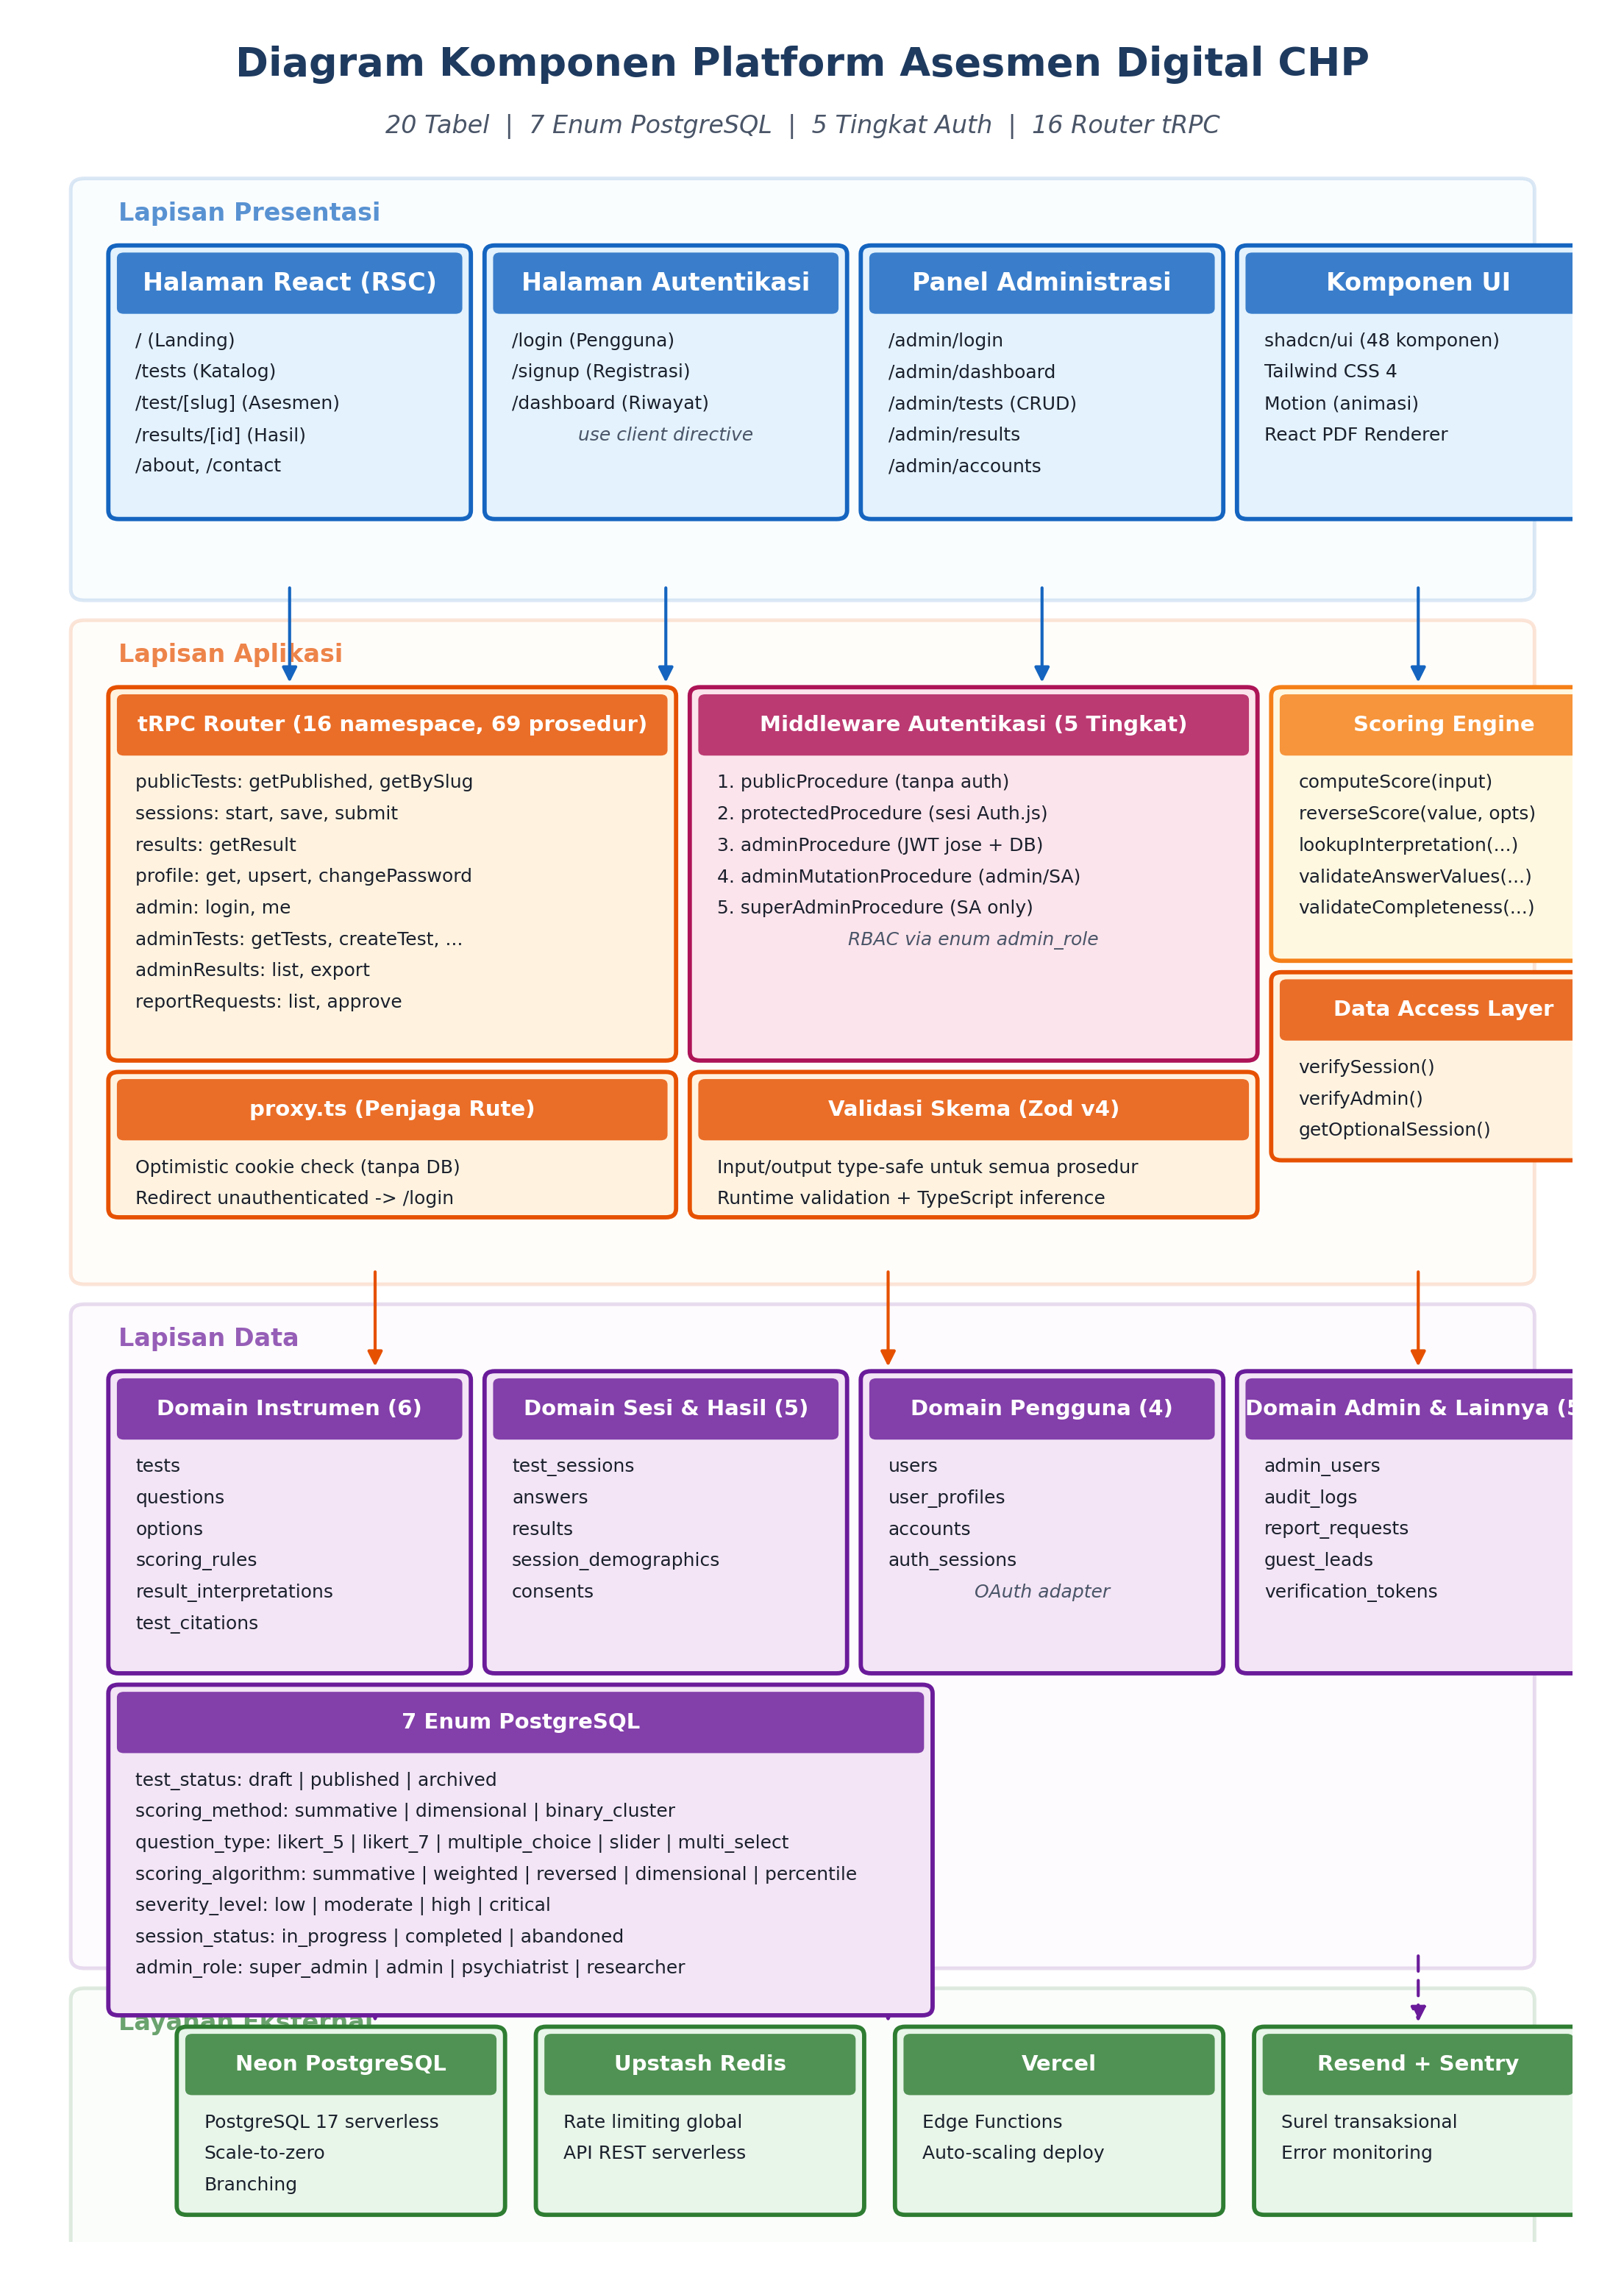
\includegraphics[width=\textwidth]{figures/gambar_3_2_komponen.png}
  \caption{Diagram Komponen Platform Asesmen Digital CHP}
  \label{fig:komponen}
\end{figure}

% [C9] Applied: 5 auth tiers in middleware description
Lapisan aplikasi terdiri atas empat modul utama:

\begin{enumerate}[leftmargin=2cm]
  \item \textit{Router} tRPC (16 \textit{namespace}) yang mengekspos 69 prosedur API.
  \item \textit{Scoring engine} (\texttt{computeScore}, \texttt{reverseScore}, \texttt{lookupInterpretation}, \texttt{validateAnswerValues}, \texttt{validateCompleteness}) yang mengandung logika komputasi skor deterministik.
  \item \textit{Middleware} autentikasi yang menerapkan lima tingkat kontrol akses: \texttt{publicProcedure}, \texttt{protectedProcedure}, \texttt{adminProcedure}, \texttt{adminMutationProcedure}, dan \texttt{superAdminProcedure}.
  \item \textit{Data Access Layer} (DAL) yang menyediakan fungsi \texttt{verifySession}, \texttt{verifyAdmin}, dan \texttt{getOptionalSession}.
\end{enumerate}

\subsection{Batas Klien-\textit{Server}}
\label{subsec:batas-klien-server}

% [C10] Applied: proxy.ts, not middleware.ts
Modul \texttt{proxy.ts} (pengganti \texttt{middleware.ts} pada Next.js 16) berfungsi sebagai penjaga rute optimistis yang membaca \textit{cookie} sesi tanpa mengakses basis data. Pemeriksaan otorisasi definitif dilakukan oleh DAL di lapisan aplikasi, sehingga keamanan bergantung pada dua lapis pertahanan yang saling menguatkan.

% ─────────────────────────────────────────────────────────────────────────────
% [C1] Applied: 16 → 20 tables; [C7] Applied: 4 missing tables added
\section{Perancangan Basis Data}
\label{sec:perancangan-db}

Skema basis data Platform CHP dirancang dengan tiga prinsip utama: (1) fleksibilitas untuk beragam instrumen psikologi; (2) pemisahan data kesehatan dari data identitas pribadi; dan (3) reproduktibilitas ilmiah melalui penyimpanan versi instrumen dan algoritma.

\subsection{Model Domain}

Skema basis data diorganisasi ke dalam lima domain:

\begin{enumerate}[leftmargin=2cm]
  \item \textbf{Domain Instrumen Asesmen} (6 tabel): mendefinisikan struktur instrumen psikometri.
  \item \textbf{Domain Sesi dan Hasil} (5 tabel): mencatat pelaksanaan asesmen.
  \item \textbf{Domain Pengguna} (4 tabel): menyediakan infrastruktur identitas dan profil.
  \item \textbf{Domain Admin dan Audit} (2 tabel): mendefinisikan pengguna administratif dan jejak audit.
  \item \textbf{Domain Permintaan dan Surel} (2 tabel): mengelola permintaan laporan dan PII.
  \item \textbf{Domain Infrastruktur Autentikasi} (1 tabel): \textit{token} verifikasi.
\end{enumerate}

\subsection{Skema Tabel}

Seluruh tabel menggunakan UUID v4 sebagai kunci primer. Tabel~\ref{tab:inventaris-tabel} menyajikan inventaris lengkap 20 tabel.

\begin{longtable}{@{}p{2.5cm} p{3cm} p{3.5cm} p{5cm}@{}}
  \caption{Inventaris Tabel Basis Data Platform CHP}
  \label{tab:inventaris-tabel} \\
  \toprule
  \textbf{Domain} & \textbf{Tabel} & \textbf{Kolom Kunci} & \textbf{Tujuan} \\
  \midrule
  \endfirsthead
  \toprule
  \textbf{Domain} & \textbf{Tabel} & \textbf{Kolom Kunci} & \textbf{Tujuan} \\
  \midrule
  \endhead
  \bottomrule
  \endfoot
  Instrumen & \texttt{tests} & id, slug, title, version & Metadata instrumen psikometri \\[0.2em]
  Instrumen & \texttt{questions} & id, test\_id, type, dimension & Butir soal dengan dimensi dan pembobotan \\[0.2em]
  Instrumen & \texttt{options} & id, question\_id, label, value & Opsi jawaban per butir soal \\[0.2em]
  Instrumen & \texttt{scoring\_rules} & id, test\_id, algorithm, config & Konfigurasi algoritma penilaian \\[0.2em]
  Instrumen & \texttt{result\_interpretations} & id, test\_id, dimension, min/max\_score & Pemetaan skor ke label interpretasi \\[0.2em]
  Instrumen & \texttt{test\_citations} & id, test\_id, type, citation, doi & Sitasi akademik per instrumen \\[0.2em]
  \midrule
  Sesi & \texttt{test\_sessions} & id, test\_id, status, claim\_token & Sesi asesmen dengan mekanisme klaim \\[0.2em]
  Sesi & \texttt{answers} & id, session\_id, question\_id, value & Respons mentah yang \textit{immutable} \\[0.2em]
  Sesi & \texttt{results} & id, session\_id, total\_score, dimension\_scores & Skor terhitung terpisah dari respons mentah \\[0.2em]
  Sesi & \texttt{session\_demographics} & session\_id, name, sex, age, province & Data demografis peserta per sesi \\[0.2em]
  Sesi & \texttt{consents} & id, session\_id, tos\_accepted, consent\_version & Persetujuan eksplisit sesuai UU PDP \\[0.2em]
  \midrule
  Pengguna & \texttt{users} & id, email, password\_hash, role & Identitas pengguna terdaftar \\[0.2em]
  Pengguna & \texttt{user\_profiles} & user\_id, display\_name, sex, age & Profil pengguna yang diperluas \\[0.2em]
  Pengguna & \texttt{accounts} & id, user\_id, provider & Tautan akun OAuth pihak ketiga \\[0.2em]
  Pengguna & \texttt{auth\_sessions} & id, session\_token, user\_id, expires & Sesi autentikasi berbasis basis data \\[0.2em]
  \midrule
  Admin & \texttt{admin\_users} & id, email, role, is\_active & Pengguna administratif dengan peran \\[0.2em]
  Admin & \texttt{audit\_logs} & id, admin\_user\_id, action, entity\_type & Jejak audit \textit{append-only} \\[0.2em]
  \midrule
  Permintaan & \texttt{report\_requests} & id, session\_id, status, requester\_type & Permintaan laporan dengan alur persetujuan \\[0.2em]
  Permintaan & \texttt{guest\_leads} & id, session\_id, encrypted\_email & PII terenkripsi AES-256-GCM \\[0.2em]
  \midrule
  Auth & \texttt{verification\_tokens} & identifier, token, expires & \textit{Token} verifikasi sekali pakai \\
\end{longtable}

Selain 20 tabel, skema mendefinisikan tujuh \textit{enum} PostgreSQL yang memastikan integritas data. Tabel~\ref{tab:enum-postgresql} mencantumkan definisinya.

\begin{table}[htbp]
  \centering
  \caption{Definisi \textit{Enum} PostgreSQL}
  \label{tab:enum-postgresql}
  \begin{tabularx}{\textwidth}{@{}l X l@{}}
    \toprule
    \textbf{Nama Enum} & \textbf{Nilai yang Diizinkan} & \textbf{Digunakan Pada} \\
    \midrule
    \texttt{test\_status} & \texttt{draft}, \texttt{published}, \texttt{archived} & \texttt{tests.status} \\
    \texttt{scoring\_method} & \texttt{summative}, \texttt{dimensional}, \texttt{binary\_cluster} & \texttt{tests.scoring\_method} \\
    \texttt{question\_type} & \texttt{likert\_5}, \texttt{likert\_7}, \texttt{multiple\_choice}, \texttt{slider}, \texttt{multi\_select} & \texttt{questions.type} \\
    \texttt{scoring\_algorithm} & \texttt{summative}, \texttt{weighted}, \texttt{reversed}, \texttt{dimensional}, \texttt{percentile} & \texttt{scoring\_rules.algorithm} \\
    \texttt{severity\_level} & \texttt{low}, \texttt{moderate}, \texttt{high}, \texttt{critical} & \texttt{result\_interpretations.severity} \\
    \texttt{session\_status} & \texttt{in\_progress}, \texttt{completed}, \texttt{abandoned} & \texttt{test\_sessions.status} \\
    \texttt{admin\_role} & \texttt{super\_admin}, \texttt{admin}, \texttt{psychiatrist}, \texttt{researcher} & \texttt{admin\_users.role} \\
    \bottomrule
  \end{tabularx}
\end{table}

\subsection{Relasi Antar-Entitas}

Gambar~\ref{fig:er-diagram} menyajikan diagram \textit{Entity-Relationship} (ER).

\begin{figure}[htbp]
  \centering
  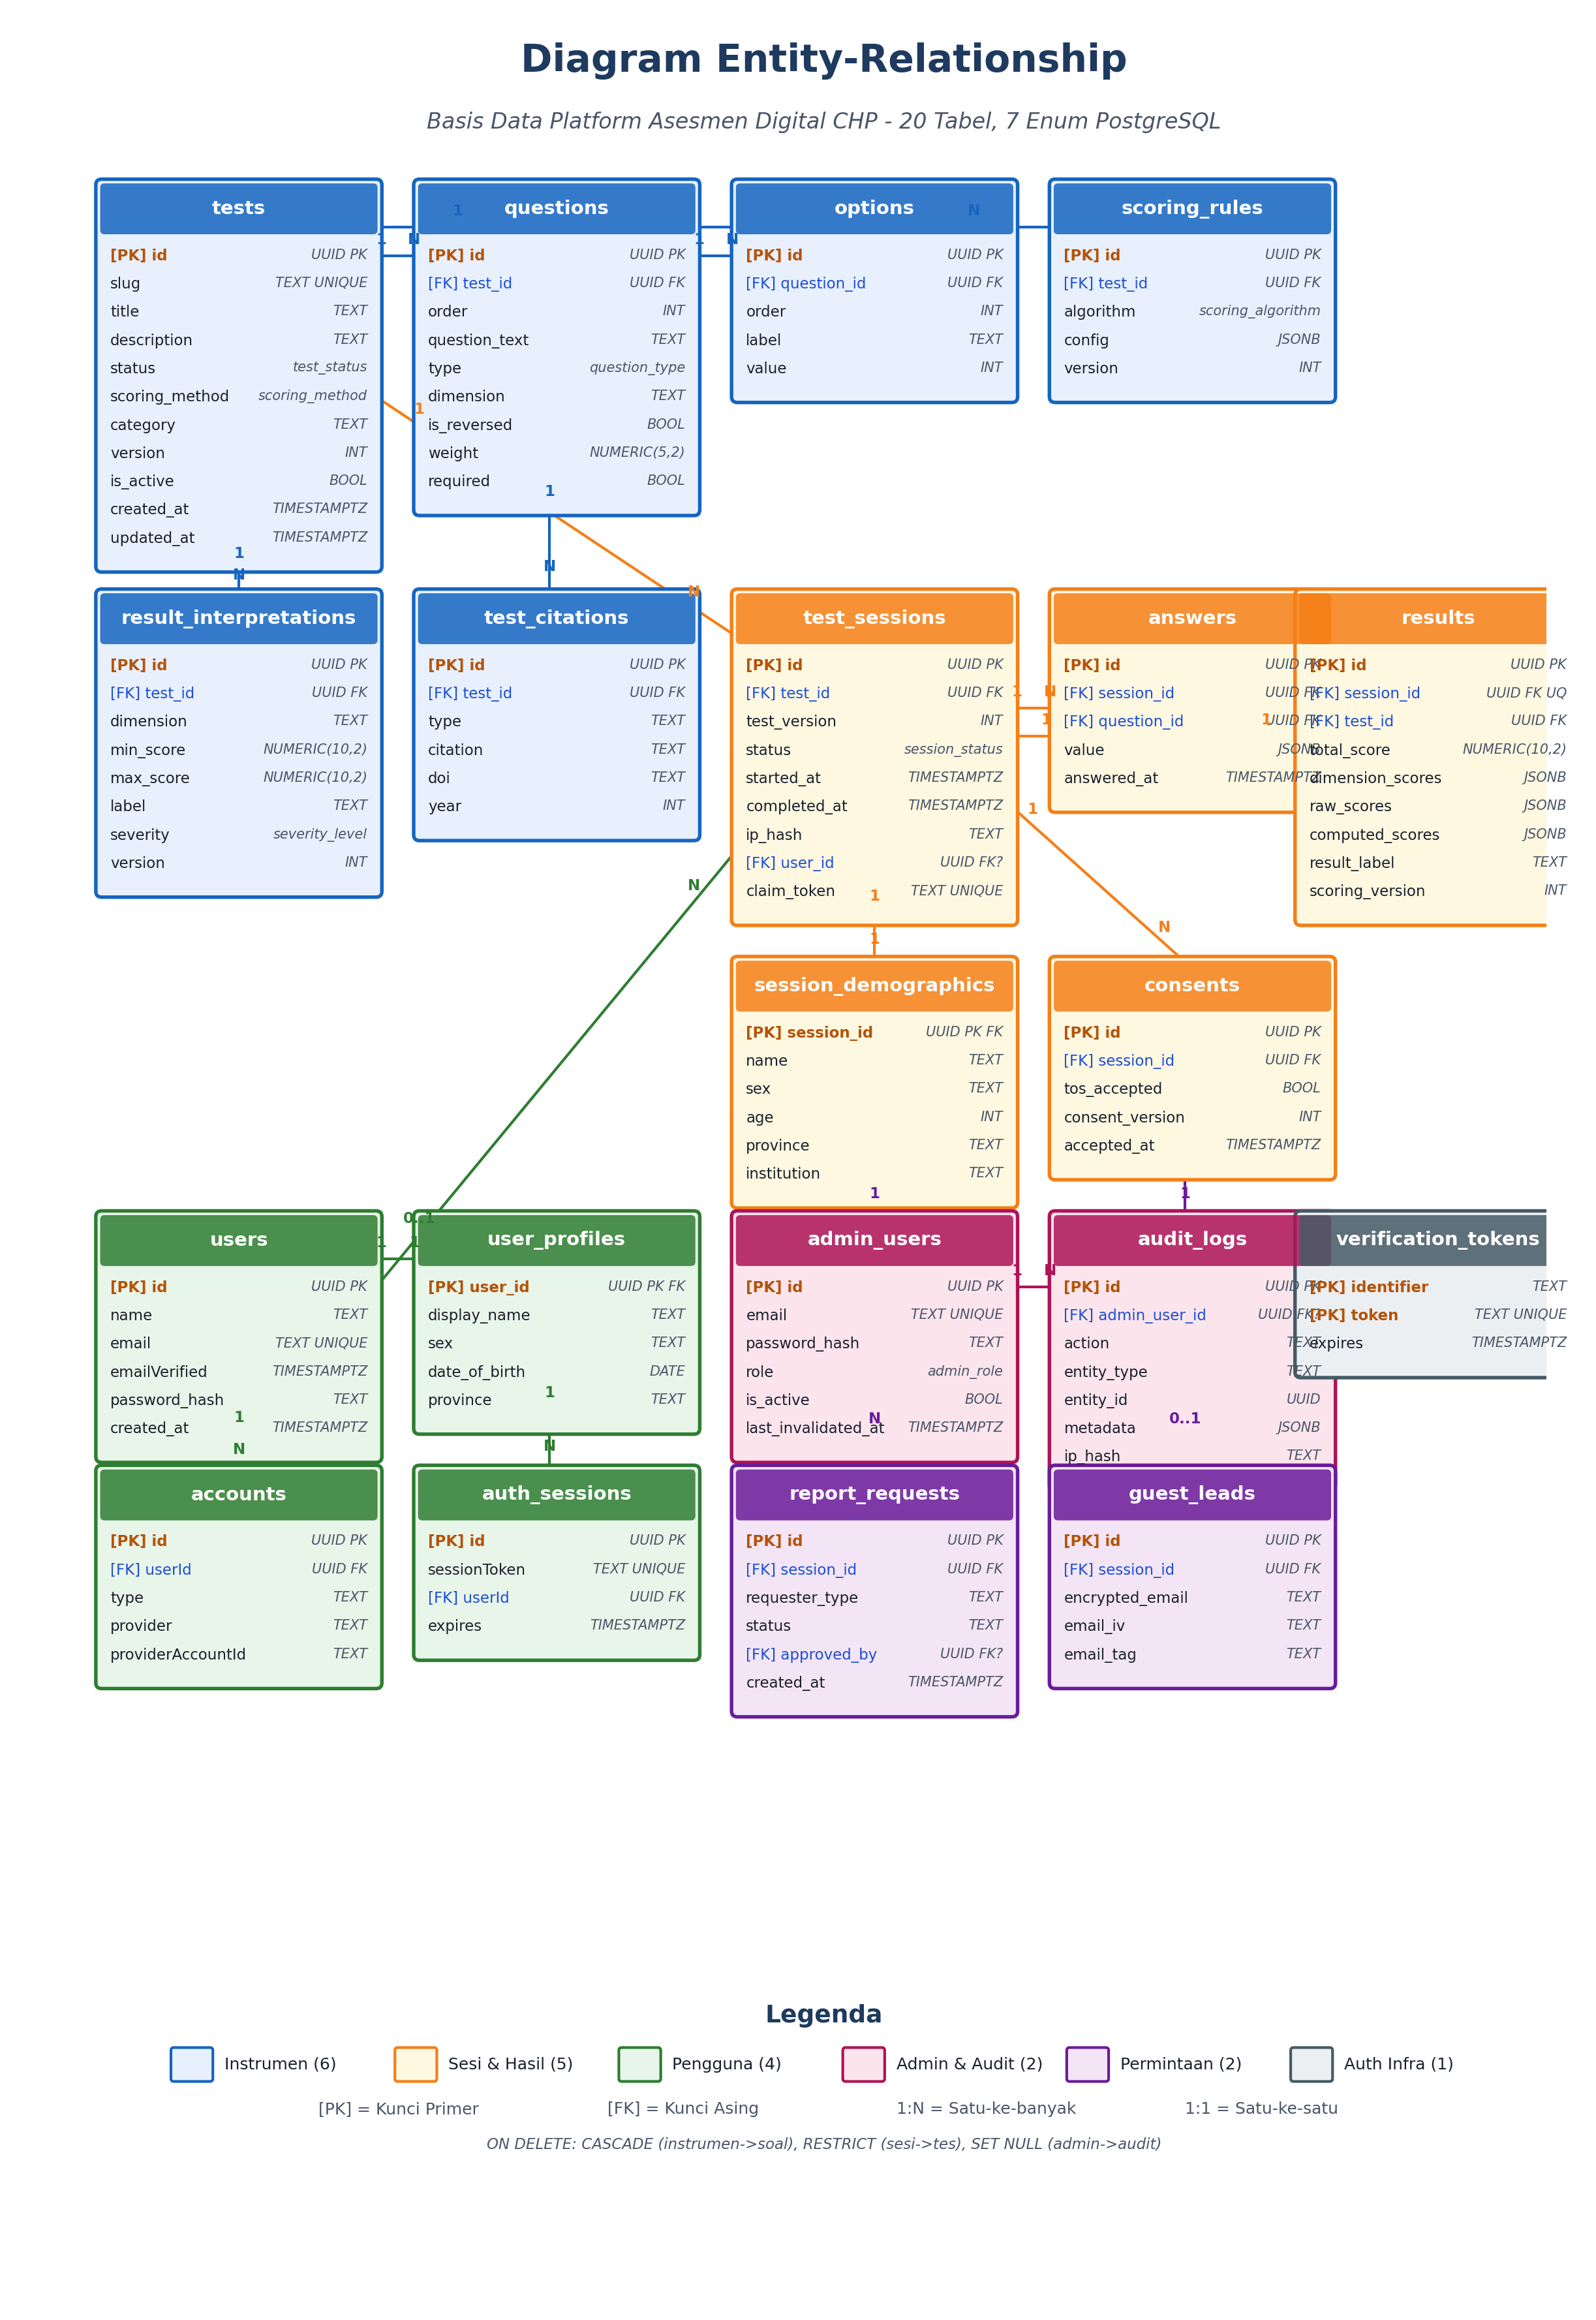
\includegraphics[width=\textwidth]{figures/gambar_3_3_er_diagram.png}
  \caption{Diagram \textit{Entity-Relationship} Basis Data Platform CHP}
  \label{fig:er-diagram}
\end{figure}

Relasi utama antar-entitas:

\begin{enumerate}[leftmargin=2cm]
  \item \texttt{tests} $\rightarrow$ \texttt{questions} $\rightarrow$ \texttt{options}: pola satu-ke-banyak bertingkat dengan \texttt{ON DELETE CASCADE}.
  \item \texttt{test\_sessions} $\rightarrow$ \texttt{answers}: \textit{constraint} unik komposit \texttt{(session\_id, question\_id)}.
  \item \texttt{test\_sessions} $\rightarrow$ \texttt{results}: relasi satu-ke-satu melalui \textit{constraint} \texttt{UNIQUE} pada \texttt{session\_id}.
  \item \texttt{test\_sessions} $\rightarrow$ \texttt{users}: \textit{foreign key} opsional (\texttt{user\_id} \textit{nullable}) dengan \texttt{ON DELETE SET NULL}.
  \item \texttt{admin\_users} $\rightarrow$ \texttt{audit\_logs}: \texttt{ON DELETE SET NULL} agar penghapusan akun admin tidak menghapus rekam jejak.
\end{enumerate}

\subsection{Keputusan Perancangan Kritis}

Empat keputusan perancangan data dengan dampak arsitektur signifikan:

\begin{enumerate}[leftmargin=2cm]
  \item \textbf{Pemisahan \texttt{answers} dan \texttt{results}}: memungkinkan \textit{re-scoring} tanpa kehilangan data historis.
  \item \textbf{JSONB untuk nilai polimorfik}: kolom \texttt{answers.value} mengakomodasi format jawaban beragam (Likert, pilihan ganda, \textit{slider}).
  \item \textbf{\textit{Claim token}}: UUID v4 dengan masa berlaku 72 jam untuk transisi anonim-ke-terdaftar; sekali pakai dan dinihilkan setelah diklaim.
  \item \textbf{Penyamaran IP dan enkripsi surel}: alamat IP di-\textit{hash} satu arah; surel dienkripsi AES-256-GCM dalam tabel \texttt{guest\_leads} yang terisolasi.
\end{enumerate}

% ─────────────────────────────────────────────────────────────────────────────
% [C3/C8] REWRITTEN: API table expanded from 8 to 22 key procedures
\section{Perancangan Antarmuka Pemrograman Aplikasi}
\label{sec:perancangan-api}

Platform CHP menggunakan tRPC sebagai protokol komunikasi. Seluruh 69 prosedur API diorganisasi ke dalam 16 \textit{router namespace}. Tabel~\ref{tab:api-publik} hingga Tabel~\ref{tab:api-admin} menyajikan inventaris prosedur yang dikelompokkan berdasarkan area fungsional.

\begin{longtable}{@{}l l c c p{5cm}@{}}
  \caption{Prosedur API Publik (Alur Asesmen)}
  \label{tab:api-publik} \\
  \toprule
  \textbf{Prosedur} & \textbf{Router} & \textbf{Tipe} & \textbf{Auth} & \textbf{Fungsi} \\
  \midrule
  \endfirsthead
  \toprule
  \textbf{Prosedur} & \textbf{Router} & \textbf{Tipe} & \textbf{Auth} & \textbf{Fungsi} \\
  \midrule
  \endhead
  \bottomrule
  \endfoot
  \texttt{getPublishedTests} & publicTests & Q & Publik & Ambil daftar tes aktif \\
  \texttt{getTestBySlug} & publicTests & Q & Publik & Ambil tes berdasarkan \textit{slug} \\
  \texttt{startSession} & sessions & M & Publik & Mulai sesi, simpan \textit{consent} + \textit{claim token} \\
  \texttt{saveDemographics} & sessions & M & Publik & Simpan data demografis \\
  \texttt{saveProgress} & sessions & M & Publik & Simpan jawaban (\textit{batch upsert}) \\
  \texttt{submitAssessment} & sessions & M & Publik & Validasi, hitung skor, simpan hasil \\
  \texttt{getResult} & results & Q & Publik & Ambil hasil asesmen \\
  \texttt{requestEmailReport} & sessions & M & Publik & Buat permintaan laporan surel \\
\end{longtable}

\begin{longtable}{@{}l l c c p{5cm}@{}}
  \caption{Prosedur API Pengguna Terdaftar}
  \label{tab:api-user} \\
  \toprule
  \textbf{Prosedur} & \textbf{Router} & \textbf{Tipe} & \textbf{Auth} & \textbf{Fungsi} \\
  \midrule
  \endfirsthead
  \toprule
  \textbf{Prosedur} & \textbf{Router} & \textbf{Tipe} & \textbf{Auth} & \textbf{Fungsi} \\
  \midrule
  \endhead
  \bottomrule
  \endfoot
  \texttt{claimSession} & sessions & M & Protected & Klaim sesi anonim ke akun \\
  \texttt{get} & profile & Q & Protected & Ambil profil pengguna \\
  \texttt{upsert} & profile & M & Protected & Simpan/perbarui profil \\
  \texttt{changePassword} & profile & M & Protected & Ganti kata sandi \\
\end{longtable}

\begin{longtable}{@{}l l c c p{5cm}@{}}
  \caption{Prosedur API Panel Administrasi}
  \label{tab:api-admin} \\
  \toprule
  \textbf{Prosedur} & \textbf{Router} & \textbf{Tipe} & \textbf{Auth} & \textbf{Fungsi} \\
  \midrule
  \endfirsthead
  \toprule
  \textbf{Prosedur} & \textbf{Router} & \textbf{Tipe} & \textbf{Auth} & \textbf{Fungsi} \\
  \midrule
  \endhead
  \bottomrule
  \endfoot
  \texttt{login} & admin & M & Publik & \textit{Login} admin, terbitkan JWT \\
  \texttt{me} & admin & Q & Admin & Profil admin aktif \\
  \texttt{stats} & adminDashboard & Q & Admin & Statistik platform \\
  \texttt{list} & adminResults & Q & Admin & Tabel hasil per instrumen \\
  \texttt{export} & adminResults & Q & Admin & Ekspor data (maks 5000 baris) \\
  \texttt{list} & reportRequests & Q & Admin & Daftar permintaan laporan \\
  \texttt{approve} & reportRequests & M & Admin & \textit{Generate} PDF + kirim surel \\
  \texttt{getTests} & adminTests & Q & Admin & Daftar instrumen \\
  \texttt{createTest} & adminTests & M & AdminMut & Buat tes baru \\
  \texttt{createAdmin} & adminAccounts & M & SuperAdmin & Buat akun admin \\
\end{longtable}

% [C9] Applied in middleware description
Setiap prosedur memanfaatkan lima tingkat \textit{middleware} autentikasi: \texttt{publicProcedure} (tanpa autentikasi), \texttt{protectedProcedure} (sesi Auth.js), \texttt{adminProcedure} (JWT admin via jose dengan validasi basis data), \texttt{adminMutationProcedure} (peran \texttt{super\_admin} atau \texttt{admin}), dan \texttt{superAdminProcedure} (khusus \texttt{super\_admin}).

% ─────────────────────────────────────────────────────────────────────────────
\section{Perancangan Alur Antarmuka Pengguna}
\label{sec:alur-ui}

Perancangan komponen antarmuka pengguna secara visual merupakan tanggung jawab anggota tim lain. Namun, perancangan alur layar (\textit{screen flow}) merupakan bagian integral dari arsitektur sistem.

\begin{figure}[htbp]
  \centering
  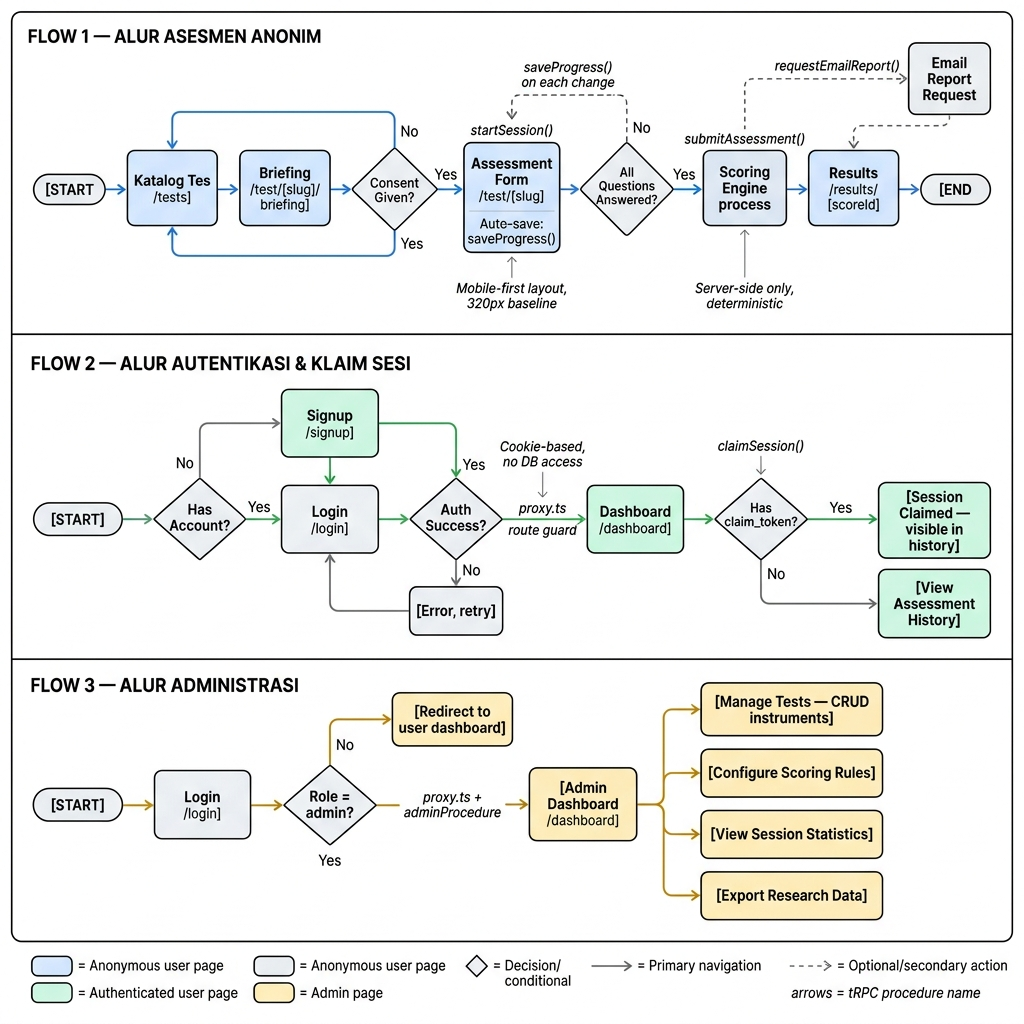
\includegraphics[width=\textwidth]{figures/gambar_3_4_alur_layar.png}
  \caption{Diagram Alur Layar Platform CHP}
  \label{fig:screen-flow}
\end{figure}

Tiga alur utama:

\begin{enumerate}[leftmargin=2cm]
  \item \textbf{Alur asesmen anonim}: \texttt{/tests} $\rightarrow$ \texttt{/test/[slug]} $\rightarrow$ \texttt{/results/[scoreId]}. Seluruh alur berjalan tanpa memerlukan akun.
  \item \textbf{Alur autentikasi dan klaim sesi}: \texttt{/signup} atau \texttt{/login} $\rightarrow$ \texttt{/dashboard}. Penjaga rute \texttt{proxy.ts} memastikan halaman terlindungi hanya diakses oleh pengguna terautentikasi.
  \item \textbf{Alur administrasi}: \texttt{/admin/login} $\rightarrow$ \texttt{/admin/dashboard} $\rightarrow$ halaman manajemen instrumen, hasil, laporan, dan akun.
\end{enumerate}
